% ============================================================
%  CHI 2026 Presentation — "Co-Adaptive Eco-Nudging"
%  Uses real paper figures from assets/
% ============================================================
\documentclass[10pt,aspectratio=169]{beamer}

% ---------- Theme ----------
\usetheme[sectionpage=none, subsectionpage=none, progressbar=frametitle]{metropolis}
\usepackage{appendixnumberbeamer}

% ---------- Mosaic-inspired palette (CHI'26 Barcelona trencadis) ----------
\definecolor{chiTeal}{HTML}{00838F}
\definecolor{chiDeep}{HTML}{004D56}
\definecolor{chiAccent}{HTML}{E8590C}
\definecolor{chiOrange}{HTML}{FF8C00}
\definecolor{chiLight}{HTML}{E0F7FA}
\definecolor{chiGray}{HTML}{455A64}
\definecolor{chiWarm}{HTML}{FFF3E0}
\definecolor{chiGreen}{HTML}{2E7D32}
\definecolor{chiPurple}{HTML}{5C3D99}
\definecolor{chiBlue}{HTML}{1565C0}
\definecolor{chiYellow}{HTML}{F9A825}
\definecolor{chiRed}{HTML}{C62828}

\setbeamercolor{frametitle}{bg=chiTeal, fg=white}
\setbeamercolor{progress bar}{fg=chiAccent}
\setbeamercolor{title separator}{fg=chiAccent}
\setbeamercolor{alerted text}{fg=chiAccent}
\setbeamercolor{background canvas}{bg=white}
\setbeamercolor{footnote}{fg=chiGray}
\setbeamercolor{page number in head/foot}{fg=chiGray}

\setbeamertemplate{frame footer}{}
\setbeamertemplate{footline}{%
  \hfill\usebeamerfont{page number in head/foot}%
  \usebeamercolor[fg]{page number in head/foot}%
  \insertframenumber\,/\,\inserttotalframenumber\kern1.2em\vskip4pt}

% ---------- Packages ----------
\usepackage{booktabs}
\usepackage{graphicx}
\usepackage{tikz}
\usetikzlibrary{shapes.geometric, arrows.meta, positioning, calc, fit,
  decorations.pathreplacing, decorations.pathmorphing, shadows.blur,
  backgrounds, fadings}
\usepackage{fontawesome5}
\usepackage{tcolorbox}
\tcbuselibrary{skins,breakable}
\usepackage{amsmath}
\usepackage{multirow}
\usepackage{array}
\usepackage{xcolor}
\usepackage{hyperref}
\usepackage{pifont}

% ---------- Mosaic corner decoration ----------
\newcommand{\mosaicCorner}[3]{%
  \begin{scope}[shift={(#1,#2)}, scale=#3, opacity=0.12]
    \fill[chiTeal]     (0,0) -- (0.4,0.1) -- (0.3,0.5) -- cycle;
    \fill[chiBlue]     (0.35,0) -- (0.8,0.15) -- (0.6,0.4) -- (0.3,0.25) -- cycle;
    \fill[chiOrange]   (0.7,0.05) -- (1.1,0.2) -- (1.0,0.55) -- (0.65,0.35) -- cycle;
    \fill[chiGreen]    (0,0.4) -- (0.35,0.45) -- (0.2,0.8) -- (-0.05,0.7) -- cycle;
    \fill[chiYellow]   (0.25,0.55) -- (0.6,0.5) -- (0.55,0.85) -- (0.15,0.9) -- cycle;
    \fill[chiAccent]   (0.5,0.45) -- (0.9,0.4) -- (0.95,0.75) -- (0.55,0.8) -- cycle;
    \fill[chiTeal!70]  (0.85,0.3) -- (1.2,0.35) -- (1.15,0.7) -- (0.8,0.65) -- cycle;
    \fill[chiBlue!60]  (0,0.75) -- (0.3,0.85) -- (0.15,1.15) -- (-0.1,1.05) -- cycle;
    \fill[chiPurple!50](0.25,0.9) -- (0.6,0.85) -- (0.55,1.2) -- (0.2,1.15) -- cycle;
  \end{scope}}

\newcommand{\sideAccent}{%
  \begin{tikzpicture}[remember picture, overlay]
    \fill[chiTeal, opacity=0.04] (current page.north west) rectangle
      ([xshift=4pt]current page.south west);
  \end{tikzpicture}}

% ---------- Custom tcolorboxes ----------
\newtcolorbox{keybox}[1][]{%
  enhanced, colback=chiLight!50, colframe=chiTeal,
  boxrule=0.8pt, arc=4pt, left=6pt, right=6pt, top=4pt, bottom=4pt,
  fonttitle=\bfseries\small\color{white}, coltitle=white, colbacktitle=chiTeal,
  drop lifted shadow, title={#1}}

\newtcolorbox{alertbox}[1][]{%
  enhanced, colback=chiWarm!60, colframe=chiAccent,
  boxrule=0.8pt, arc=4pt, left=6pt, right=6pt, top=4pt, bottom=4pt,
  fonttitle=\bfseries\small\color{white}, coltitle=white, colbacktitle=chiAccent,
  drop lifted shadow, title={#1}}

\newtcolorbox{findingbox}{%
  enhanced, colback=white, colframe=chiTeal!40,
  boxrule=0.6pt, arc=3pt, left=6pt, right=6pt, top=3pt, bottom=3pt,
  drop lifted shadow, borderline west={2.5pt}{0pt}{chiTeal}}

\newcommand{\emphmark}[1]{\textcolor{chiAccent}{\textbf{#1}}}

% ---------- Title info ----------
\title{\texorpdfstring{Co-Adaptive Eco-Nudging}{Co-Adaptive Eco-Nudging}}
\subtitle{A Privacy-Preserving Contextual Bandit with User-Taught Preferences in Everyday Browsing}
\author{Guangrui Fan\textsuperscript{1*} \quad Dandan Liu\textsuperscript{2} \quad Lihu Pan\textsuperscript{1}}
\institute{}
\date{}

\begin{document}

% ============================================================
%  TITLE SLIDE
% ============================================================
{
\setbeamertemplate{footline}{}
\begin{frame}[plain,noframenumbering]
\begin{tikzpicture}[remember picture, overlay]
  \fill[chiDeep] (current page.north west) rectangle (current page.south east);
  \fill[chiTeal, opacity=0.6] (current page.north west) rectangle
    ([yshift=-4.5cm]current page.north east);
  \mosaicCorner{-6.5}{3.8}{1.8}
  \mosaicCorner{5.2}{3.2}{1.4}
  \mosaicCorner{-5.0}{-3.5}{1.2}
  \mosaicCorner{6.0}{-2.8}{1.0}
  \node[anchor=north west, rounded corners=4pt, fill=white,
    inner xsep=5pt, inner ysep=4pt]
    at ([xshift=10mm, yshift=-6mm]current page.north west)
    {
\includegraphics[height=1.2cm]{assets/chi2026-logo.png}};
  \node[anchor=west, text=white, font=\LARGE\bfseries, text width=12cm]
    at ([xshift=14mm, yshift=14mm]current page.west)
    {Co-Adaptive Eco-Nudging};
  \node[anchor=west, text=white!85, font=\normalsize, text width=12cm]
    at ([xshift=14mm, yshift=4mm]current page.west)
    {A Privacy-Preserving Contextual Bandit with};
  \node[anchor=west, text=white!85, font=\normalsize, text width=12cm]
    at ([xshift=14mm, yshift=-2mm]current page.west)
    {User-Taught Preferences in Everyday Browsing};
  \draw[chiAccent, line width=1.5pt]
    ([xshift=14mm, yshift=-8mm]current page.west) --
    ([xshift=100mm, yshift=-8mm]current page.west);
  \node[anchor=west, text=white!90, font=\small]
    at ([xshift=14mm, yshift=-15mm]current page.west)
    {Guangrui Fan\textsuperscript{1*} \quad Dandan Liu\textsuperscript{2} \quad Lihu Pan\textsuperscript{1}};
  \node[anchor=west, text=white!65, font=\scriptsize, text width=11cm]
    at ([xshift=14mm, yshift=-21mm]current page.west)
    {\textsuperscript{1}Taiyuan University of Science and Technology, China \quad
     \textsuperscript{2}Faculty of Arts \& Social Sciences, Universiti Malaya, Malaysia};
  \fill[white] ([yshift=0mm]current page.south west) rectangle
    ([yshift=16mm]current page.south east);
  \node[anchor=south west] at ([xshift=14mm, yshift=2mm]current page.south west)
    {
\includegraphics[height=1.1cm]{assets/tyust-logo.png}};
  \node[anchor=south] at ([xshift=-20mm, yshift=2.5mm]current page.south)
    {
\includegraphics[height=1.0cm]{assets/chi2026-logo.png}};
  \node[anchor=south] at ([xshift=20mm, yshift=2mm]current page.south)
    {
\includegraphics[height=1.0cm]{assets/acm-logo.png}};
  \node[anchor=south east] at ([xshift=-14mm, yshift=3mm]current page.south east)
    {
\includegraphics[height=0.9cm]{assets/sigchi-logo.png}};
  \node[rounded corners=3pt, fill=chiAccent, text=white, font=\footnotesize\bfseries,
    inner xsep=8pt, inner ysep=3pt, anchor=south]
    at ([yshift=18mm]current page.south)
    {CHI 2026 ~\textbullet~ April 13--17 ~\textbullet~ Barcelona, Spain};
\end{tikzpicture}
\end{frame}
}

% ============================================================
%  SECTION 1: MOTIVATION
% ============================================================
{
\setbeamertemplate{footline}{}
\begin{frame}[plain,noframenumbering]
\begin{tikzpicture}[remember picture, overlay]
  \fill[chiTeal] (current page.north west) rectangle
    ([yshift=-3.5cm]current page.north east);
  \mosaicCorner{-6}{1.5}{1.5}
  \mosaicCorner{5.5}{1.0}{1.2}
  \node[anchor=west, text=white, font=\huge\bfseries]
    at ([xshift=16mm, yshift=-1.75cm]current page.north west) {1};
  \node[anchor=west, text=white, font=\Large]
    at ([xshift=28mm, yshift=-1.75cm]current page.north west)
    {Motivation \& Research Questions};
  \draw[chiAccent, line width=2pt]
    ([xshift=16mm, yshift=-2.8cm]current page.north west) --
    ([xshift=70mm, yshift=-2.8cm]current page.north west);
  \node[anchor=north west, text=chiGray, font=\small\itshape, text width=12cm]
    at ([xshift=16mm, yshift=-4.2cm]current page.north west)
    {Can digital eco-nudges be both effective and respectful of user autonomy?};
\end{tikzpicture}
\end{frame}
}

% ============================================================

\begin{frame}{Background: The Digital Eco-Nudging Challenge}
\begin{columns}[T]
\begin{column}{0.62\textwidth}
\begin{keybox}[\faGlobe~~ The Problem Space]
\scriptsize
Digital services (browsing, streaming, file transfers, printing) mediate growing shares of aggregate energy demand and emissions. SHCI has explored eco-feedback and persuasive technologies, yet:
\begin{itemize}
  \item Focusing on ``small changes'' is insufficient without structural attention~[Brynjarsdottir et al.\ 2012]
  \item Rebound effects can erase efficiency gains~[Walzberg 2020]
  \item Prior nudging evaluations show heterogeneous effects, short horizons, and evaluation confounds~[Caraban et al.\ 2019]
\end{itemize}
\end{keybox}
\begin{alertbox}[\faExclamationTriangle~~ Key Tensions]
\scriptsize
\begin{itemize}
  \item Personalization increases relevance but risks \emphmark{surveillance \& manipulation}~[Puntoni et al.\ 2021]
  \item Poorly timed/frequent prompts cause annoyance and attrition~[Valta et al.\ 2022]
  \item Interventions themselves consume resources --- net impact rarely reported~[Preist et al.\ 2019]
\end{itemize}
\end{alertbox}
\end{column}
\begin{column}{0.35\textwidth}
\begin{keybox}[\faLightbulb~~ Our Approach]
\scriptsize
\textbf{Personalization without profiling:} a privacy-preserving, on-device contextual bandit that learns \emph{when} to act and \emph{when} to do nothing.
\end{keybox}
\vspace{2pt}
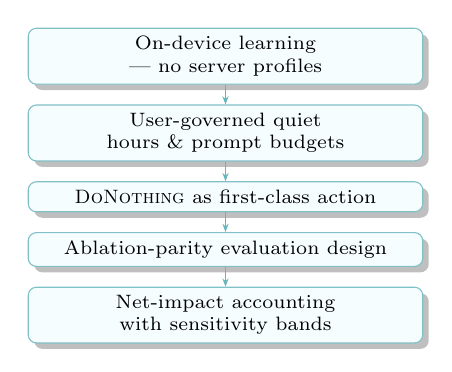
\begin{tikzpicture}[
  node distance=0.25cm,
  block/.style={rounded corners=3pt, draw=chiTeal!50, fill=chiLight!30,
    text width=4.8cm, align=center, font=\scriptsize, inner sep=3pt, drop shadow}]
  \node[block] (a) {On-device learning --- no server profiles};
  \node[block, below=of a] (b) {User-governed quiet hours \& prompt budgets};
  \node[block, below=of b] (c) {\textsc{DoNothing} as first-class action};
  \node[block, below=of c] (d) {Ablation-parity evaluation design};
  \node[block, below=of d] (e) {Net-impact accounting with sensitivity bands};
  \draw[-{Stealth[length=3pt]}, chiTeal!60] (a) -- (b);
  \draw[-{Stealth[length=3pt]}, chiTeal!60] (b) -- (c);
  \draw[-{Stealth[length=3pt]}, chiTeal!60] (c) -- (d);
  \draw[-{Stealth[length=3pt]}, chiTeal!60] (d) -- (e);
\end{tikzpicture}
\end{column}
\end{columns}
\end{frame}

% ============================================================

\begin{frame}{Gaps \& Research Questions}
\sideAccent
\vspace{2pt}
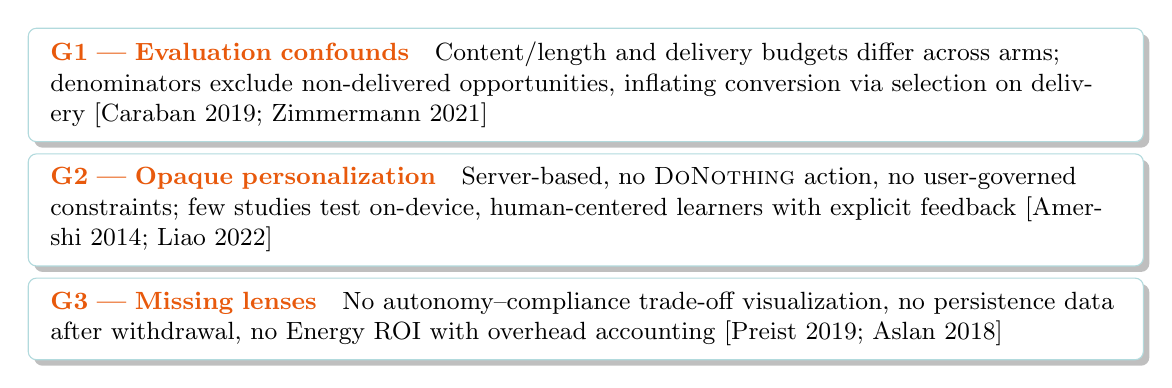
\begin{tikzpicture}[
  gap/.style={rounded corners=3pt, fill=white, draw=chiTeal!30,
    text width=13.6cm, align=left, font=\small,
    inner xsep=8pt, inner ysep=5pt, drop shadow}]
  \node[gap] (g1) at (0,0) {
    \textcolor{chiAccent}{\textbf{G1 --- Evaluation confounds}}~~
    Content/length and delivery budgets differ across arms; denominators exclude non-delivered opportunities, inflating conversion via selection on delivery~[Caraban~2019; Zimmermann~2021]};
  \node[gap, below=4pt of g1] (g2) {
    \textcolor{chiAccent}{\textbf{G2 --- Opaque personalization}}~~
    Server-based, no \textsc{DoNothing} action, no user-governed constraints; few studies test on-device, human-centered learners with explicit feedback~[Amershi~2014; Liao~2022]};
  \node[gap, below=4pt of g2] (g3) {
    \textcolor{chiAccent}{\textbf{G3 --- Missing lenses}}~~
    No autonomy--compliance trade-off visualization, no persistence data after withdrawal, no Energy ROI with overhead accounting~[Preist~2019; Aslan~2018]};
\end{tikzpicture}
\vspace{4pt}
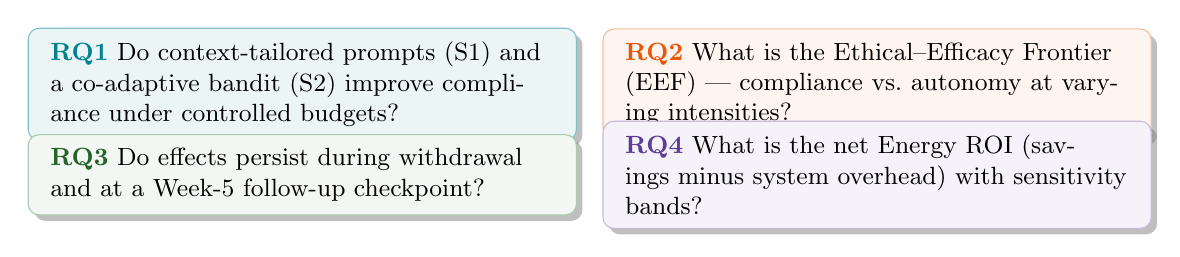
\begin{tikzpicture}[
  rq/.style={rounded corners=4pt, text width=6.4cm, align=left, font=\small,
    inner xsep=8pt, inner ysep=5pt, drop shadow}]
  \node[rq, fill=chiTeal!8, draw=chiTeal!50] (r1) at (0,0) {
    \textcolor{chiTeal}{\textbf{RQ1}} Do context-tailored prompts (S1) and a co-adaptive bandit (S2) improve compliance under controlled budgets?};
  \node[rq, fill=chiAccent!6, draw=chiAccent!40] (r2) at (7.3,0) {
    \textcolor{chiAccent}{\textbf{RQ2}} What is the Ethical--Efficacy Frontier (EEF) --- compliance vs.\ autonomy at varying intensities?};
  \node[rq, fill=chiGreen!6, draw=chiGreen!40] (r3) at (0,-1.15) {
    \textcolor{chiGreen!80!black}{\textbf{RQ3}} Do effects persist during withdrawal and at a Week-5 follow-up checkpoint?};
  \node[rq, fill=chiPurple!6, draw=chiPurple!35] (r4) at (7.3,-1.15) {
    \textcolor{chiPurple}{\textbf{RQ4}} What is the net Energy ROI (savings minus system overhead) with sensitivity bands?};
\end{tikzpicture}
\end{frame}

% ============================================================
%  SECTION 2: SYSTEM
% ============================================================
{
\setbeamertemplate{footline}{}
\begin{frame}[plain,noframenumbering]
\begin{tikzpicture}[remember picture, overlay]
  \fill[chiTeal] (current page.north west) rectangle
    ([yshift=-3.5cm]current page.north east);
  \mosaicCorner{-6}{1.5}{1.5}
  \mosaicCorner{5.5}{1.0}{1.2}
  \node[anchor=west, text=white, font=\huge\bfseries]
    at ([xshift=16mm, yshift=-1.75cm]current page.north west) {2};
  \node[anchor=west, text=white, font=\Large]
    at ([xshift=28mm, yshift=-1.75cm]current page.north west)
    {System: Co-Adaptive Nudge Pipeline};
  \draw[chiAccent, line width=2pt]
    ([xshift=16mm, yshift=-2.8cm]current page.north west) --
    ([xshift=70mm, yshift=-2.8cm]current page.north west);
  \node[anchor=north west, text=chiGray, font=\small\itshape, text width=12cm]
    at ([xshift=16mm, yshift=-4.2cm]current page.north west)
    {Privacy-preserving, on-device contextual bandit with learned restraint};
\end{tikzpicture}
\end{frame}
}

% ============================================================

\begin{frame}{Pipeline Architecture}
\sideAccent
\vspace{-4pt}
\begin{columns}[T]
\begin{column}{0.37\textwidth}
\begin{keybox}[\faLayerGroup~~ Three Phases]
\scriptsize
\textbf{Phase 1 --- Onboarding:} Goal selection (carbon, cost, performance, curiosity), persuasion style (Analyst/Coach/Pragmatist), quiet hours, daily prompt budget $C{\in}\{0..4\}$, per-behavior opt-outs.\\[3pt]
\textbf{Phase 2 --- Adaptive Engine:} On-device Thompson sampling over $\mathcal{A}{=}\{\textsc{DoNothing}\}{\cup}\{\text{Targets}{\times}\text{Styles}\}$, subject to hard budget/quiet-hour constraints.\\[3pt]
\textbf{Phase 3 --- Feedback \& XAI:} Template-based \emph{Why this?} explanations; one-tap feedback (Helpful $+1$, Annoying $-1$, Wrong time $-0.5$) shapes future decisions.
\end{keybox}
\end{column}
\begin{column}{0.62\textwidth}
\vspace{-2pt}
\begin{center}
  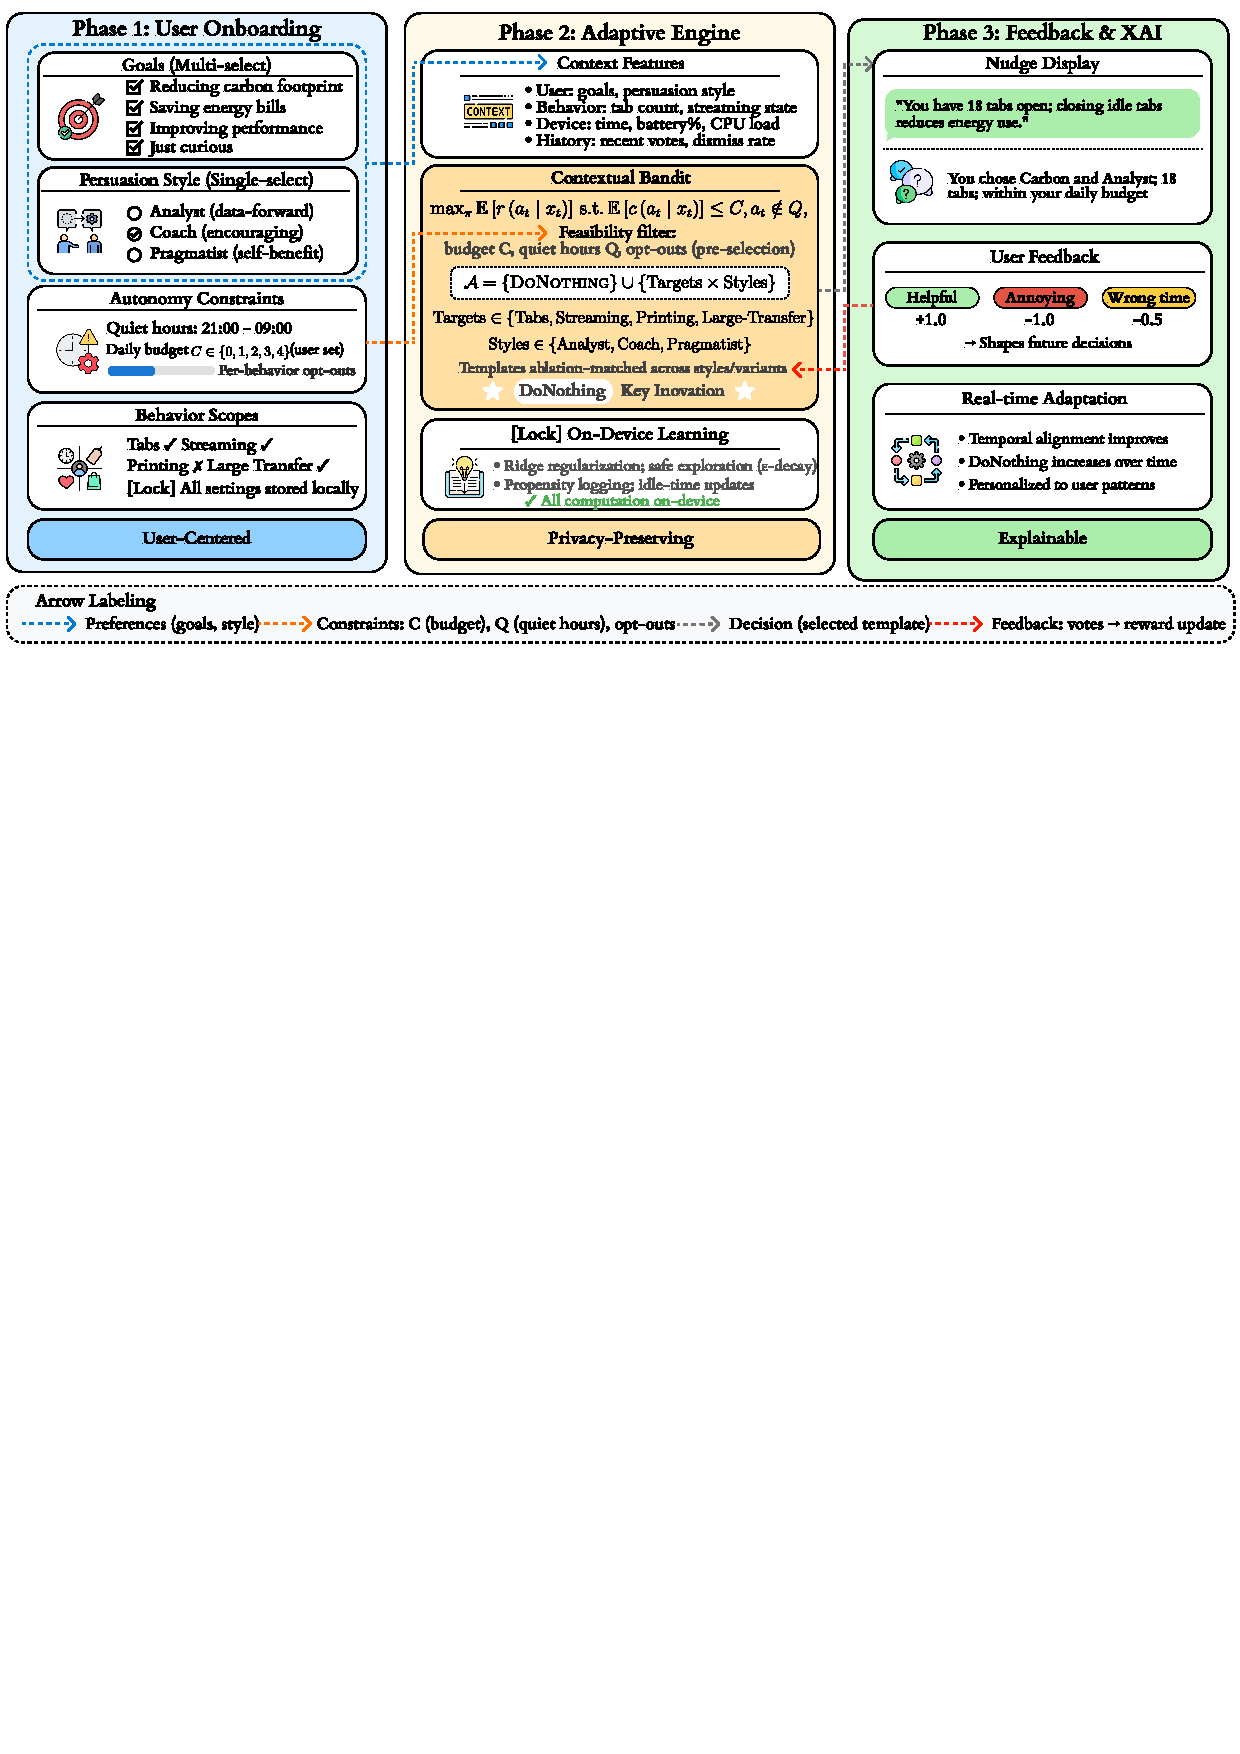
\includegraphics[width=\linewidth, height=0.78\textheight, keepaspectratio]{assets/pipeline_diagram.pdf}
\end{center}
\vspace{3pt}
\begin{findingbox}
\scriptsize
All computation and data remain \textbf{on device}. No server-side profile. Users can pause, adjust, or opt out per behavior at any time.
\end{findingbox}
\end{column}
\end{columns}
\end{frame}

% ============================================================

\begin{frame}{System Details: Target Behaviors \& Privacy}
\sideAccent
\vspace{0pt}
\begin{columns}[T]
\begin{column}{0.45\textwidth}
\begin{tikzpicture}[
  behav/.style={rounded corners=3pt, fill=white, draw=chiTeal!35,
    text width=5.8cm, align=left, font=\scriptsize,
    inner xsep=6pt, inner ysep=4pt, drop shadow}]
  \node[behav] (b1) at (0,0) {
    \textcolor{chiTeal}{\faVideo~~\textbf{Streaming Quality}} --- Monitors HTML5 \texttt{videoWidth}$\times$\texttt{videoHeight}; flags sessions $\ge$720p as HD. Compliance: switch to $\le$480p within 5\,min.};
  \node[behav, below=4pt of b1] (b2) {
    \textcolor{chiBlue}{\faLayerGroup~~\textbf{Tab Management}} --- Tracks concurrent tab count. Opportunity: tabs $>$ 12 (cohort 75th pctl). Compliance: reduce by $\ge$2 or below threshold within 10\,min.};
  \node[behav, below=4pt of b2] (b3) {
    \textcolor{chiGreen!80!black}{\faPrint~~\textbf{Printing}} --- Hooks Ctrl/Cmd+P and \texttt{window.print()}. Compliance: dialog closed without printing within 60\,s, no job within 10\,min.};
  \node[behav, below=4pt of b3] (b4) {
    \textcolor{chiPurple}{\faCloud~~\textbf{Large File Transfers}} --- webRequest monitors Content-Length; flags $\ge$500\,MB. Compliance: cancel within 2\,min, no retry within 30\,min.};
\end{tikzpicture}
\end{column}
\begin{column}{0.53\textwidth}
\begin{alertbox}[\faLock~~ Privacy by Design]
\scriptsize
\begin{itemize}\setlength\itemsep{2pt}
  \item \textbf{No page content captured} --- only event metadata (tab counts, resolution, print invocations, request sizes)
  \item \textbf{On-device inference \& storage} --- model parameters $(\hat{\theta}_a, A_a)$ never leave the browser
  \item \textbf{Ephemeral counters} with bounded retention (last-7 votes, last-24h dismiss rate)
  \item \textbf{Idle-time updates} minimize foreground contention
  \item \textbf{Hard autonomy constraints} enforced before action selection
\end{itemize}
\end{alertbox}
\begin{keybox}[\faCogs~~ Ablation Parity]
\scriptsize
Messages matched across conditions on \textbf{length} ($\pm$5\%, mean 82.4 chars), \textbf{reading level} (grade 7--9), and \textbf{valence} ($\kappa{=}0.82$). Context-tailored differs only by a minimal factual token (\texttt{\{tab\_count\}}, \texttt{\{today\_hd\_mins\}}).
\end{keybox}
\end{column}
\end{columns}
\end{frame}

% ============================================================

\begin{frame}{Key Technical Details: Bandit Formulation}
\vspace{0pt}
\begin{columns}[T]
\begin{column}{0.52\textwidth}
\begin{keybox}[\faChartLine~~ Constrained Objective]
\small
At each decision time $t$, select $a_t \in \mathcal{A}$ to maximize:
\[
\max_{\pi}\;\mathbb{E}[r(a_t \mid x_t)] \quad\text{s.t.}\quad \mathbb{E}[c(a_t \mid x_t)] \le C,\; a_t \notin \mathcal{Q}
\]

\scriptsize
\begin{itemize}\setlength\itemsep{1pt}
  \item $r_t = \mathbb{I}[\text{compliance}] + \text{vote}(v_t)$ ~(composite reward)
  \item $c_t = \mathbb{I}[a_t \neq \textsc{DoNothing}]$ ~(unit cost per delivery)
  \item $C$ = user-set daily prompt budget (0--4)
  \item $\mathcal{Q}$ = quiet hours (median 21:00--09:00)
\end{itemize}
\end{keybox}
\vspace{3pt}
\begin{findingbox}
\scriptsize
\textbf{Thompson Sampling (Study 2):} Draw $\tilde{\theta}_a \sim \mathcal{N}(\hat{\theta}_a, \sigma^2 A_a^{-1})$ with $\lambda{=}0.5$, $\sigma^2{=}0.25$; select $\arg\max_a \tilde{\theta}_a^\top x_t$ among feasible actions. Safe exploration: $\varepsilon_t$ decays from 0.20 to 0.05 over first 5 prompts.
\end{findingbox}
\end{column}
\begin{column}{0.46\textwidth}
\begin{keybox}[\faDatabase~~ Context Features $x_t \in \mathbb{R}^d$]
\scriptsize
\begin{itemize}\setlength\itemsep{0pt}
  \item \textbf{User-seeded:} goal vector (one-hot); persuasion style
  \item \textbf{Behavioral state:} tab count; streaming state \& resolution; recent large transfer; time since last prompt (per target)
  \item \textbf{Temporal/device:} time-of-day, day-of-week; battery \%; coarse CPU load; session length
  \item \textbf{Ephemeral history:} rolling Helpful/Annoying counts (last-7); last-24h dismiss rate
\end{itemize}
\end{keybox}
\vspace{1pt}
\begin{alertbox}[\faHandPaper~~ \textsc{DoNothing} Action]
\scriptsize
Always present in $\mathcal{A}$ and frequently optimal once the model learns user-specific patterns. Enables \emphmark{algorithmic restraint}: the learner treats attention as a \textbf{scarce, user-governed good}, not a resource to exhaust.
\vspace{1pt}
\textbf{Study 2:} \textsc{DoNothing} grew from \emphmark{38\%} (Days 1--3) to \emphmark{68\%} (Days 10--14) of all decision points.
\end{alertbox}
\end{column}
\end{columns}
\end{frame}

% ============================================================
%  SECTION 3: STUDY 1
% ============================================================
{
\setbeamertemplate{footline}{}
\begin{frame}[plain,noframenumbering]
\begin{tikzpicture}[remember picture, overlay]
  \fill[chiTeal] (current page.north west) rectangle
    ([yshift=-3.5cm]current page.north east);
  \mosaicCorner{-6}{1.5}{1.5}
  \mosaicCorner{5.5}{1.0}{1.2}
  \node[anchor=west, text=white, font=\huge\bfseries]
    at ([xshift=16mm, yshift=-1.75cm]current page.north west) {3};
  \node[anchor=west, text=white, font=\Large]
    at ([xshift=28mm, yshift=-1.75cm]current page.north west)
    {Study 1: Context-Tailored vs.\ Generic};
  \draw[chiAccent, line width=2pt]
    ([xshift=16mm, yshift=-2.8cm]current page.north west) --
    ([xshift=70mm, yshift=-2.8cm]current page.north west);
  \node[anchor=north west, text=chiGray, font=\small\itshape, text width=12cm]
    at ([xshift=16mm, yshift=-4.2cm]current page.north west)
    {$N{=}178$, 3-arm between-subjects, 2-week field study with ablation parity};
  \node[rounded corners=3pt, fill=chiAccent, text=white, font=\small\bfseries,
    inner xsep=10pt, inner ysep=4pt]
    at ([xshift=-25mm, yshift=-1.75cm]current page.north east) {$N{=}178$};
\end{tikzpicture}
\end{frame}
}

% ============================================================

\begin{frame}{Study 1 --- Design \& Participants}
\vspace{-2pt}
\begin{columns}[T]
\begin{column}{0.55\textwidth}
\vspace{0pt}
\begin{keybox}[\faFlask~~ 3-Arm Between-Subjects Design]
\scriptsize
\begin{itemize}
  \item \textbf{Control} ($n{=}59$): no prompts, logging only
  \item \textbf{Generic} ($n{=}59$): ablation-matched generic messages
  \item \textbf{Context-Tailored} ($n{=}60$): identical messages + minimal factual personalization token
\end{itemize}
\vspace{1pt}
\tiny
\textbf{Duration:} 2 weeks ~\textbullet~ \textbf{Randomization:} permuted blocks (6--9)\\
\textbf{Budget parity:} $C{=}3$/day, inter-prompt $\ge$2\,h, per-behavior cool-down 6\,h, quiet hours 21:00--09:00\\
\textbf{Recruitment:} university lists (43\%), community forums (17\%), online postings (40\%)
\end{keybox}
\vspace{0pt}
\begin{alertbox}[\faCheckCircle~~ Ablation Parity Controls]
\scriptsize
\begin{itemize}
  \item Identical delivery budgets and cool-downs across arms
  \item Message length within $\pm$5\%, reading level matched
  \item Opportunity denominators include \emph{all} detected opportunities, not just delivered prompts
  \item Study 1 fixed tone to Analyst across all arms
\end{itemize}
\end{alertbox}
\end{column}
\begin{column}{0.48\textwidth}
{\scriptsize
\begin{table}
\centering
\renewcommand{\arraystretch}{0.95}
\resizebox{\linewidth}{!}{%
\begin{tabular}{@{}lccc@{}}
\toprule
& \textbf{Ctrl} & \textbf{Gen} & \textbf{Ctx} \\
& ($n$=59) & ($n$=59) & ($n$=60) \\
\midrule
Age (yrs) & 31.9\small{$\pm$8.6} & 32.6\small{$\pm$8.9} & 32.4\small{$\pm$8.3} \\
Women\,/\,Men\,/\,NB+ (\%) & 48/49/3 & 49/48/3 & 48/50/2 \\
Platform Win/mac/Lin & 61/36/3 & 63/34/3 & 63/32/5 \\
Tech prof.\ (1--7) & 5.0\small{$\pm$1.1} & 5.1\small{$\pm$1.2} & 5.2\small{$\pm$1.0} \\
Env.\ awareness (1--5) & 3.44\small{$\pm$.63} & 3.54\small{$\pm$.62} & 3.57\small{$\pm$.67} \\
\midrule
HD stream (min/d) & 96.1\small{$\pm$49} & 92.7\small{$\pm$52} & 92.6\small{$\pm$51} \\
Concurrent tabs & 10.9\small{$\pm$4.2} & 10.5\small{$\pm$4.0} & 10.8\small{$\pm$4.1} \\
Prints/week & 2.3\small{$\pm$1.5} & 2.2\small{$\pm$1.4} & 2.1\small{$\pm$1.3} \\
Transfers (GB/wk) & 2.9\small{$\pm$2.0} & 2.7\small{$\pm$1.8} & 2.8\small{$\pm$1.9} \\
\bottomrule
\end{tabular}
}
\end{table}
}
\vspace{2pt}
\begin{findingbox}
\scriptsize
No significant baseline differences between arms: HD min $F(2,175){=}0.27$, $p{=}.76$; tabs $F{=}0.41$, $p{=}.66$; printing $F{=}0.38$, $p{=}.68$; transfers $H{=}0.88$, $p{=}.64$. Env.\ awareness: small non-significant trend ($F{=}2.56$, $p{=}.08$); adjusted in all models.
\end{findingbox}
\end{column}
\end{columns}
\end{frame}

% ============================================================

\begin{frame}{Study 1 --- Daily Compliance Results (RQ1)}
\begin{columns}[T]
\begin{column}{0.56\textwidth}
\vspace{0pt}
\begin{center}
  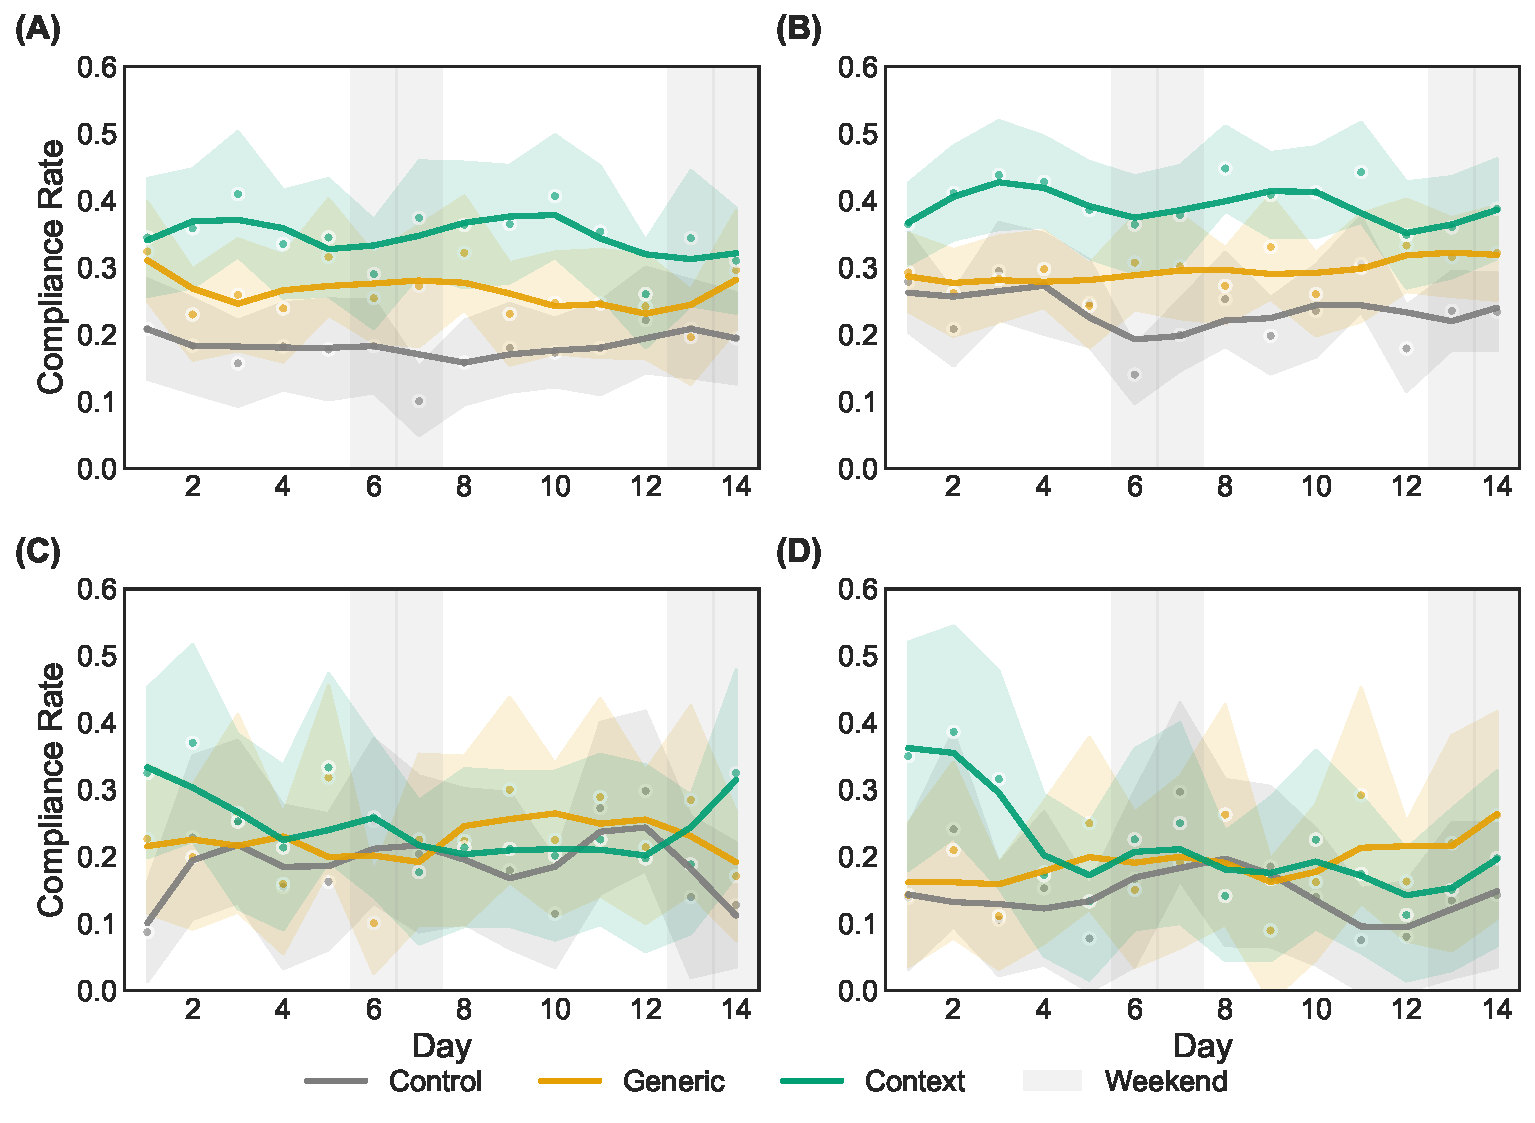
\includegraphics[width=\linewidth, height=0.62\textheight, keepaspectratio]{assets/fig3_s1_daily_compliance_enhanced.pdf}
\end{center}
\end{column}
\begin{column}{0.42\textwidth}
\vspace{0pt}
{\scriptsize
\renewcommand{\arraystretch}{0.92}
\begin{tabular}{@{}lcccc@{}}
\toprule
\textbf{Behavior} & \textbf{Ctrl} & \textbf{Gen} & \textbf{Ctx} \\
\midrule
Streaming & .19 & .27 & \textbf{.35} \\
Tabs      & .24 & .31 & \textbf{.39} \\
Printing  & .18 & .22 & \textbf{.24} \\
Lg.\ Transfer & .16 & .20 & \textbf{.23} \\
\bottomrule
\end{tabular}
}
\vspace{2pt}
\begin{findingbox}
\scriptsize
\textbf{Streaming:} Ctx--Ctrl \emphmark{+16.1\,pp} [10.8, 21.5], $p{<}.001$; Ctx--Gen \emphmark{+8.0\,pp} [3.1, 12.9], $p{=}.002$\\[2pt]
\textbf{Tabs:} Ctx--Ctrl \emphmark{+14.1\,pp} [9.7, 20.0], $p{<}.001$; Ctx--Gen \emphmark{+7.7\,pp} [2.8, 12.6], $p{=}.003$\\[2pt]
\textbf{Printing:} Ctx--Ctrl +6.1\,pp [1.2, 11.0], $p{=}.021$; Ctx--Gen +1.9\,pp, $p{=}.24$ (ns)\\[2pt]
\textbf{Transfer:} Ctx--Ctrl +7.0\,pp [2.0, 12.0], $p{=}.014$; Ctx--Gen +3.0\,pp, $p{=}.067$ (ns)
\end{findingbox}
\end{column}
\end{columns}

\vspace{3pt}
\begin{alertbox}[\faBalanceScale~~ Autonomy--Burden Slope]
\scriptsize
Autonomy slope: $\hat{\eta}_1 = -0.22$ pts/prompt/day [--0.28, --0.16], $p{<}.001$. No slope difference between Generic and Context ($\Delta$slope = --0.03, $p{=}.31$). \emphmark{Autonomy costs accrue with intensity, not tailoring.}
\end{alertbox}
\end{frame}

% ============================================================

\begin{frame}{Study 1 --- Behavior-Level Outcomes \& Heterogeneity}
\begin{columns}[T]
\begin{column}{0.54\textwidth}
\begin{keybox}[\faChartBar~~ Behavior-Level Changes (adjusted $\Delta$ from baseline/day)]
\scriptsize
\renewcommand{\arraystretch}{1.1}
\begin{tabular}{@{}lccl@{}}
\toprule
\textbf{Outcome} & \textbf{Ctrl} & \textbf{Ctx} & \textbf{Ctx--Ctrl} \\
\midrule
HD min/day & --2.9 & --13.1 & \textbf{--10.2} [$p{<}.001$] \\
Concurrent tabs & --0.3 & --1.1 & \textbf{--0.8} [$p{<}.001$] \\
Prints/day & --0.03 & --0.09 & \textbf{--0.06} [$p{=}.042$] \\
GB/day & --0.04 & --0.12 & \textbf{--0.08} [$p{=}.024$] \\
\bottomrule
\end{tabular}
\end{keybox}
\vspace{4pt}
\begin{findingbox}
\scriptsize
\textbf{Ctx--Gen (behavior-level):} HD min --5.9\,pp [--10.3, --1.5], $p{=}.008$; tabs --0.4 [--0.7, --0.1], $p{=}.014$. Printing and transfers: directionally positive but smaller and not BH-significant for Ctx--Gen.
\end{findingbox}
\end{column}
\begin{column}{0.5\textwidth}
\begin{alertbox}[\faUsers~~ Heterogeneity (Heavy Users)]
\scriptsize
\textbf{Heavy streamers} (top tertile baseline HD):
\begin{itemize}\setlength\itemsep{1pt}
  \item Ctx--Gen Streaming: \emphmark{+11.9\,pp} [5.2, 18.6], $p{<}.01$
  \item vs.\ +4.7\,pp [0.2, 9.2] for remaining participants
\end{itemize}
\vspace{1pt}
\textbf{Heavy tab users} (top tertile):
\begin{itemize}\setlength\itemsep{1pt}
  \item Ctx--Gen Tabs: \emphmark{+9.8\,pp} [3.7, 15.9], $p{=}.002$
  \item vs.\ +5.1\,pp [0.4, 9.8] for remaining
\end{itemize}
\vspace{1pt}
No consistent moderation by environmental awareness after BH correction.
\end{alertbox}
\vspace{1pt}
\begin{keybox}[\faCheckDouble~~ Robustness]
\scriptsize
Probit link: $\le$1.2\,pp shift. Random slopes/AR(1): $\le$1.3\,pp. Dropping each behavior from pooled index: max 22\% reduction, significance preserved. Power: $\ge$80\% for $\ge$5--6\,pp differences.
\end{keybox}
\end{column}
\end{columns}
\end{frame}

% ============================================================
%  SECTION 4: STUDY 2
% ============================================================
{
\setbeamertemplate{footline}{}
\begin{frame}[plain,noframenumbering]
\begin{tikzpicture}[remember picture, overlay]
  \fill[chiTeal] (current page.north west) rectangle
    ([yshift=-3.5cm]current page.north east);
  \mosaicCorner{-6}{1.5}{1.5}
  \mosaicCorner{5.5}{1.0}{1.2}
  \node[anchor=west, text=white, font=\huge\bfseries]
    at ([xshift=16mm, yshift=-1.75cm]current page.north west) {4};
  \node[anchor=west, text=white, font=\Large]
    at ([xshift=28mm, yshift=-1.75cm]current page.north west)
    {Study 2: Co-Adaptive Bandit};
  \draw[chiAccent, line width=2pt]
    ([xshift=16mm, yshift=-2.8cm]current page.north west) --
    ([xshift=70mm, yshift=-2.8cm]current page.north west);
  \node[anchor=north west, text=chiGray, font=\small\itshape, text width=12cm]
    at ([xshift=16mm, yshift=-4.2cm]current page.north west)
    {$N{=}54$, Bandit vs Rule, ABA(W) design with withdrawal and follow-up};
  \node[rounded corners=3pt, fill=chiAccent, text=white, font=\small\bfseries,
    inner xsep=10pt, inner ysep=4pt]
    at ([xshift=-25mm, yshift=-1.75cm]current page.north east) {$N{=}54$};
\end{tikzpicture}
\end{frame}
}

% ============================================================

\begin{frame}{Study 2 --- Design \& ABA(W) Protocol}
\vspace{-2pt}
\begin{columns}[T]
\begin{column}{0.52\textwidth}
\vspace{0pt}
\begin{keybox}[\faFlask~~ 2-Arm Between-Subjects Design]
\scriptsize
\begin{itemize}[nosep, leftmargin=*]
  \item \textbf{Co-Adaptive Bandit} ($n{=}27$): on-device Thompson sampling with \textsc{DoNothing}, user-governed constraints
  \item \textbf{Rule-Based Context-Tailored} ($n{=}27$): Study 1 threshold triggers with identical budgets/cool-downs
  \item \textbf{Same} nudge UI, \emph{Why this?}, and feedback buttons --- only the \emphmark{decision policy} differs
\end{itemize}
\end{keybox}
\end{column}
\begin{column}{0.46\textwidth}
\vspace{0pt}
\begin{keybox}[\faUserCog~~ Onboarding Choices (Study 2)]
\tiny
\textbf{Goals (multi-select):} Carbon 72\%, Cost 44\%, Performance 31\%, Curious 22\%\\[1pt]
\textbf{Persuasion style:} Analyst 43\%, Coach 37\%, Pragmatist 20\%\\[1pt]
\textbf{Quiet hours:} median 21:00--09:00\\[1pt]
\textbf{Daily budget $C$:} median 3, IQR [2,\,3]\\[1pt]
Per-behavior opt-outs: $<$5\% (none for Streaming/Tabs)
\end{keybox}
\vspace{2pt}
{\tiny
\renewcommand{\arraystretch}{0.88}
\begin{tabular}{@{}lcc@{}}
\toprule
& \textbf{Bandit} ($n$=27) & \textbf{Rule} ($n$=27) \\
\midrule
Age range & \multicolumn{2}{c}{18--55+}\\
Women/Men/NB+ & \multicolumn{2}{c}{46\%/50\%/4\%}\\
HD stream (min/d) & \multicolumn{2}{c}{95.6 $\pm$ 48.7}\\
Budget $C$ (mean) & 2.81 & 2.78 \\
Realized prompts/d & 2.09$\pm$.61 & 2.14$\pm$.58 \\
\bottomrule
\end{tabular}
}
\end{column}
\end{columns}
\vspace{4pt}
\centering
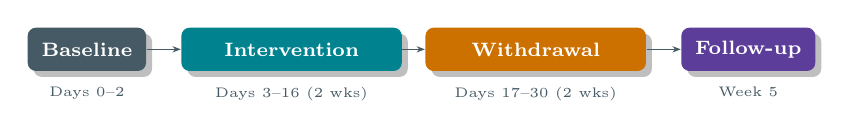
\begin{tikzpicture}[
  phase/.style={rounded corners=3pt, minimum height=0.55cm,
    text=white, font=\scriptsize\bfseries, inner xsep=5pt, drop shadow},
  label/.style={font=\tiny, text=chiGray}]
  \node[phase, fill=chiGray, minimum width=1.4cm] (bl) at (0,0) {Baseline};
  \node[phase, fill=chiTeal, minimum width=2.8cm] (int) at (2.6,0) {Intervention};
  \node[phase, fill=chiOrange!80!black, minimum width=2.8cm] (wd) at (5.7,0) {Withdrawal};
  \node[phase, fill=chiPurple, minimum width=1.6cm] (fu) at (8.4,0) {Follow-up};
  \node[label, below=2pt of bl] {Days 0--2};
  \node[label, below=2pt of int] {Days 3--16 (2 wks)};
  \node[label, below=2pt of wd] {Days 17--30 (2 wks)};
  \node[label, below=2pt of fu] {Week 5};
  \draw[-{Stealth[length=3pt]}, chiGray] (bl) -- (int);
  \draw[-{Stealth[length=3pt]}, chiGray] (int) -- (wd);
  \draw[-{Stealth[length=3pt]}, chiGray] (wd) -- (fu);
\end{tikzpicture}
\vspace{1pt}
\begin{findingbox}
\scriptsize
Budgets balanced: $t(52){=}0.19$, $p{=}.85$. Realized intensity balanced: $t(52){=}{-}0.32$, $p{=}.75$. Fair test at \emphmark{equal friction}.
\end{findingbox}
\end{frame}

% ============================================================

\begin{frame}{Study 2 --- ABA(W) Timeline \& Primary Efficacy (RQ1)}
\sideAccent
\vspace{-4pt}
\begin{columns}[T]
\begin{column}{0.56\textwidth}
\begin{center}
  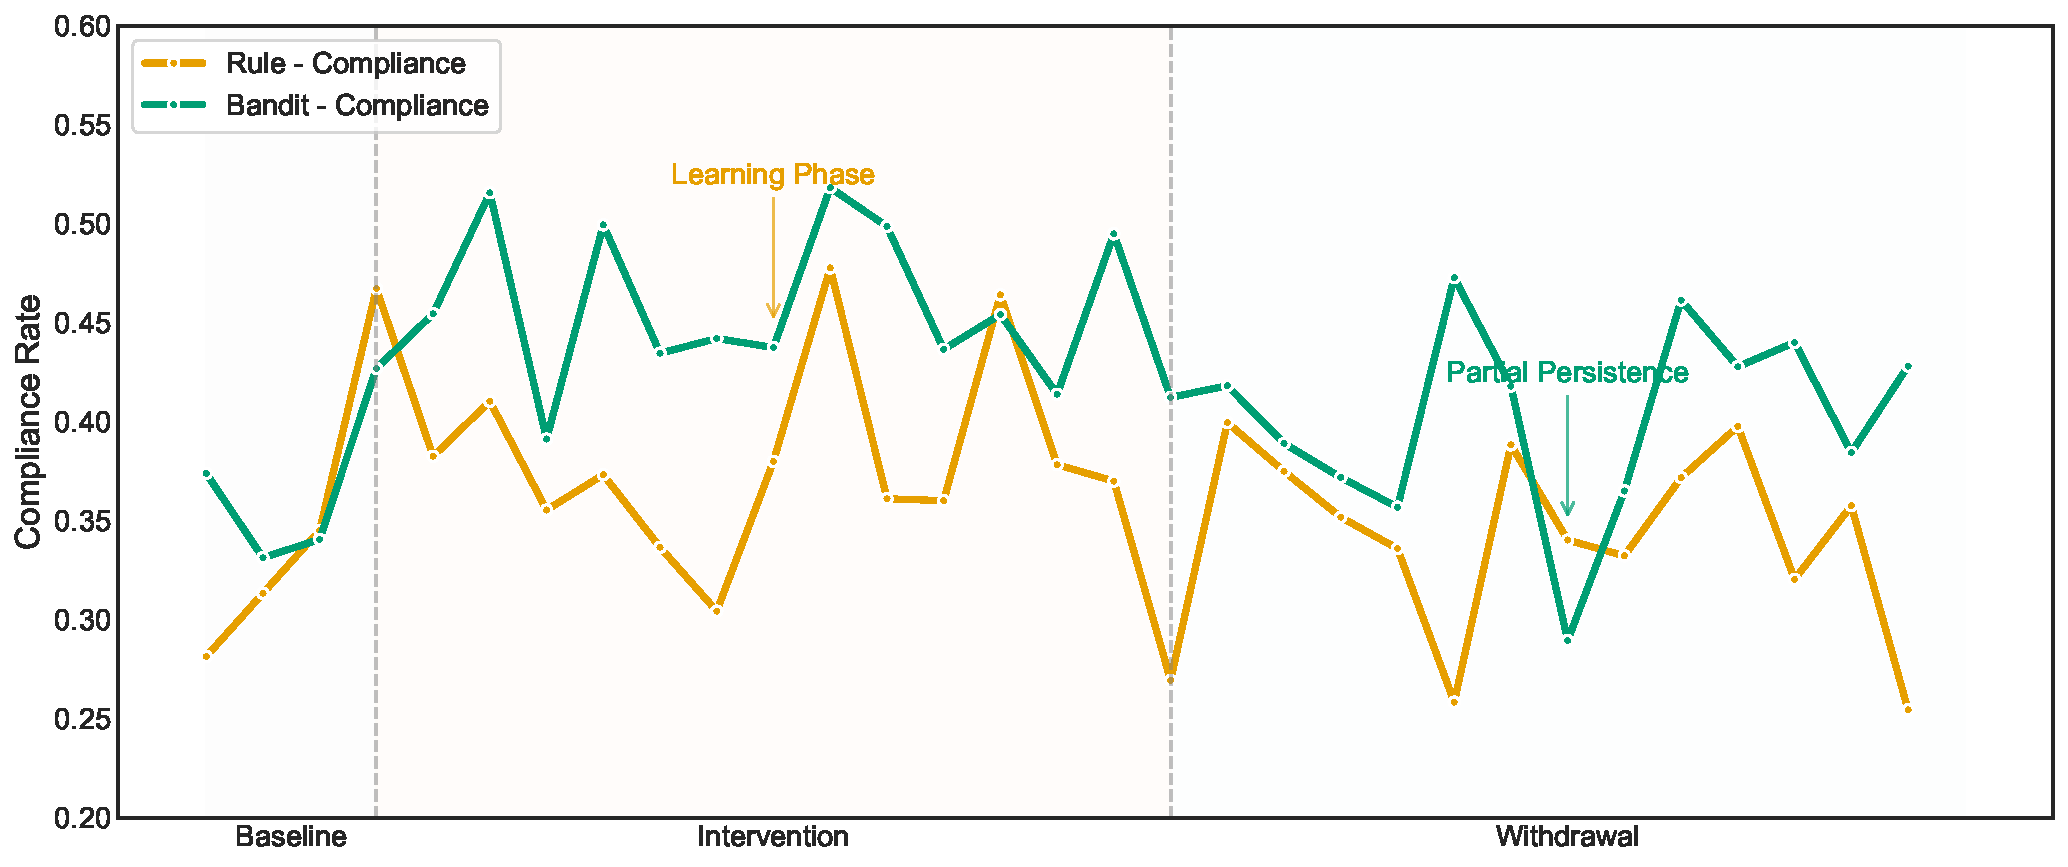
\includegraphics[width=\linewidth, height=0.78\textheight, keepaspectratio]{assets/fig5_s2_timeline_enhanced.pdf}
{\scriptsize
\renewcommand{\arraystretch}{1.0}
\begin{tabular}{@{}lccc@{}}
\toprule
\textbf{Behavior} & \textbf{Rule} & \textbf{Bandit} & $\Delta$\,pp \\
\midrule
Streaming & .36 & \textbf{.43} & \emphmark{+6.9} \\
Tabs      & .40 & \textbf{.47} & \emphmark{+7.2} \\
Printing  & .25 & .28 & +3.4 \\
Lg.\ Transfer & .23 & .27 & +3.7 \\
\bottomrule
\end{tabular}
}
\end{center}
\end{column}
\begin{column}{0.42\textwidth}
\vspace{2pt}
\begin{findingbox}
\scriptsize
\textbf{Streaming:} Bandit--Rule \emphmark{+6.9\,pp} [2.1, 11.7], $p{=}.006$\\[2pt]
\textbf{Tabs:} Bandit--Rule \emphmark{+7.2\,pp} [2.4, 12.0], $p{=}.004$\\[2pt]
\textbf{Printing:} +3.4\,pp [--0.8, 7.6], $p{=}.11$ (ns)\\[2pt]
\textbf{Transfer:} +3.7\,pp [--0.5, 7.9], $p{=}.09$ (ns)
\end{findingbox}
\vspace{3pt}
\begin{keybox}[\faChartBar~~ Behavior-Level Outcomes]
\scriptsize
HD min/day: Bandit --18.5 vs Rule --11.2; diff \emphmark{--7.3} [--13.1, --1.5], $p{=}.015$\\[2pt]
Tabs/day: Bandit --1.4 vs Rule --0.9; diff \emphmark{--0.5} [--1.0, 0.0], $p{=}.047$\\[2pt]
Prints/day: --0.03, $p{=}.43$ (ns)\\
GB/day: --0.05, $p{=}.31$ (ns)
\end{keybox}
\end{column}
\end{columns}
\end{frame}

% ============================================================

\begin{frame}{Study 2 --- \textsc{DoNothing} Learning Dynamics}
\vspace{-2pt}
\begin{columns}[T]
\begin{column}{0.55\textwidth}
\vspace{0pt}
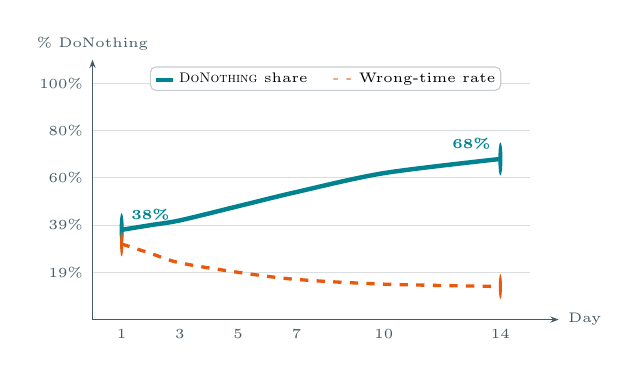
\begin{tikzpicture}[
  xscale=0.37, yscale=3.0,
  every node/.style={font=\scriptsize}]
  % Axes
  \draw[-{Stealth[length=3pt]}, chiGray] (0,0) -- (16,0) node[right] {\tiny Day};
  \draw[-{Stealth[length=3pt]}, chiGray] (0,0) -- (0,1.1) node[above] {\tiny \% DoNothing};
  % Grid
  \foreach \y in {0.2,0.4,0.6,0.8,1.0} {
    \draw[chiGray!20] (0,\y) -- (15,\y);
    \pgfmathtruncatemacro{\lab}{\y*100}
    \node[left, font=\tiny, chiGray] at (0,\y) {\lab\%};
  }
  \foreach \x in {1,3,5,7,10,14} {
    \node[below, font=\tiny, chiGray] at (\x,0) {\x};
  }
  % DoNothing curve
  \draw[chiTeal, line width=1.6pt, smooth]
    plot coordinates {(1,0.38) (2,0.40) (3,0.42) (5,0.48) (7,0.54) (10,0.62) (14,0.68)};
  \fill[chiTeal] (1,0.38) circle (2pt) node[above right, font=\tiny\bfseries] {38\%};
  \fill[chiTeal] (14,0.68) circle (2pt) node[above left, font=\tiny\bfseries] {68\%};
  % Wrong-time curve
  \draw[chiAccent, line width=1.2pt, dashed, smooth]
    plot coordinates {(1,0.32) (2,0.28) (3,0.24) (5,0.20) (7,0.17) (10,0.15) (14,0.14)};
  \fill[chiAccent] (1,0.32) circle (1.5pt);
  \fill[chiAccent] (14,0.14) circle (1.5pt);
  % Legend
  \node[rounded corners=2pt, fill=white, draw=chiGray!30, inner sep=2pt, font=\tiny]
    at (8,1.02) {
    \textcolor{chiTeal}{\rule{6pt}{1.5pt}} \textsc{DoNothing} share \quad
    \textcolor{chiAccent}{- -} Wrong-time rate};
\end{tikzpicture}
\vspace{2pt}
\begin{findingbox}
\scriptsize
\textbf{Learned restraint:} \textsc{DoNothing} grew from \emphmark{38\%} to \emphmark{68\%} of decision points over 14 days. Wrong-time votes dropped as the bandit learned \emph{when not to interrupt}.
\end{findingbox}
\begin{findingbox}
\scriptsize
\textbf{Off-policy check:} IPS uplift: Streaming +6.5\,pp (SE 2.6), Tabs +6.9\,pp (SE 2.5) --- aligns with GLMM estimates. Weights well-behaved (max 9.7, mean 1.13, ESS 0.91$\times$nominal).
\end{findingbox}
\end{column}
\begin{column}{0.48\textwidth}
\vspace{0pt}
\begin{keybox}[\faClock~~ Temporal Alignment]
\small
Share of prompts in hours without subsequent \emph{Wrong time} votes: rose from \emphmark{68\%} to \emphmark{86\%} over intervention.\\[3pt]
Mixed-effects logistic model (controlling for intensity): residual Bandit-over-time reduction in Wrong-time votes: OR $= 0.86$ [0.77, 0.96], suggesting genuine temporal alignment beyond habituation.
\end{keybox}
\vspace{2pt}
\begin{alertbox}[\faThumbsUp~~ Feedback Drives Learning]
\scriptsize
\begin{itemize}
  \item \textbf{Helpful} votes predicted higher next-day compliance:
    OR = \emphmark{1.41} [1.12, 1.78], $p{=}.003$
  \item \textbf{Annoying} votes predicted compliance reduction:
    OR = \emphmark{0.74} [0.59, 0.92], $p{=}.007$
\end{itemize}
\end{alertbox}
\end{column}
\end{columns}
\end{frame}

% ============================================================
%  SECTION 5: NEW LENSES
% ============================================================
{
\setbeamertemplate{footline}{}
\begin{frame}[plain,noframenumbering]
\begin{tikzpicture}[remember picture, overlay]
  \fill[chiTeal] (current page.north west) rectangle
    ([yshift=-3.5cm]current page.north east);
  \mosaicCorner{-6}{1.5}{1.5}
  \mosaicCorner{5.5}{1.0}{1.2}
  \node[anchor=west, text=white, font=\huge\bfseries]
    at ([xshift=16mm, yshift=-1.75cm]current page.north west) {5};
  \node[anchor=west, text=white, font=\Large]
    at ([xshift=28mm, yshift=-1.75cm]current page.north west)
    {EEF, Persistence \& Energy ROI};
  \draw[chiAccent, line width=2pt]
    ([xshift=16mm, yshift=-2.8cm]current page.north west) --
    ([xshift=70mm, yshift=-2.8cm]current page.north west);
  \node[anchor=north west, text=chiGray, font=\small\itshape, text width=12cm]
    at ([xshift=16mm, yshift=-4.2cm]current page.north west)
    {Making autonomy--compliance trade-offs and net environmental impact visible};
\end{tikzpicture}
\end{frame}
}

% ============================================================

\begin{frame}{Ethical--Efficacy Frontier (EEF) --- RQ2}
\begin{center}
  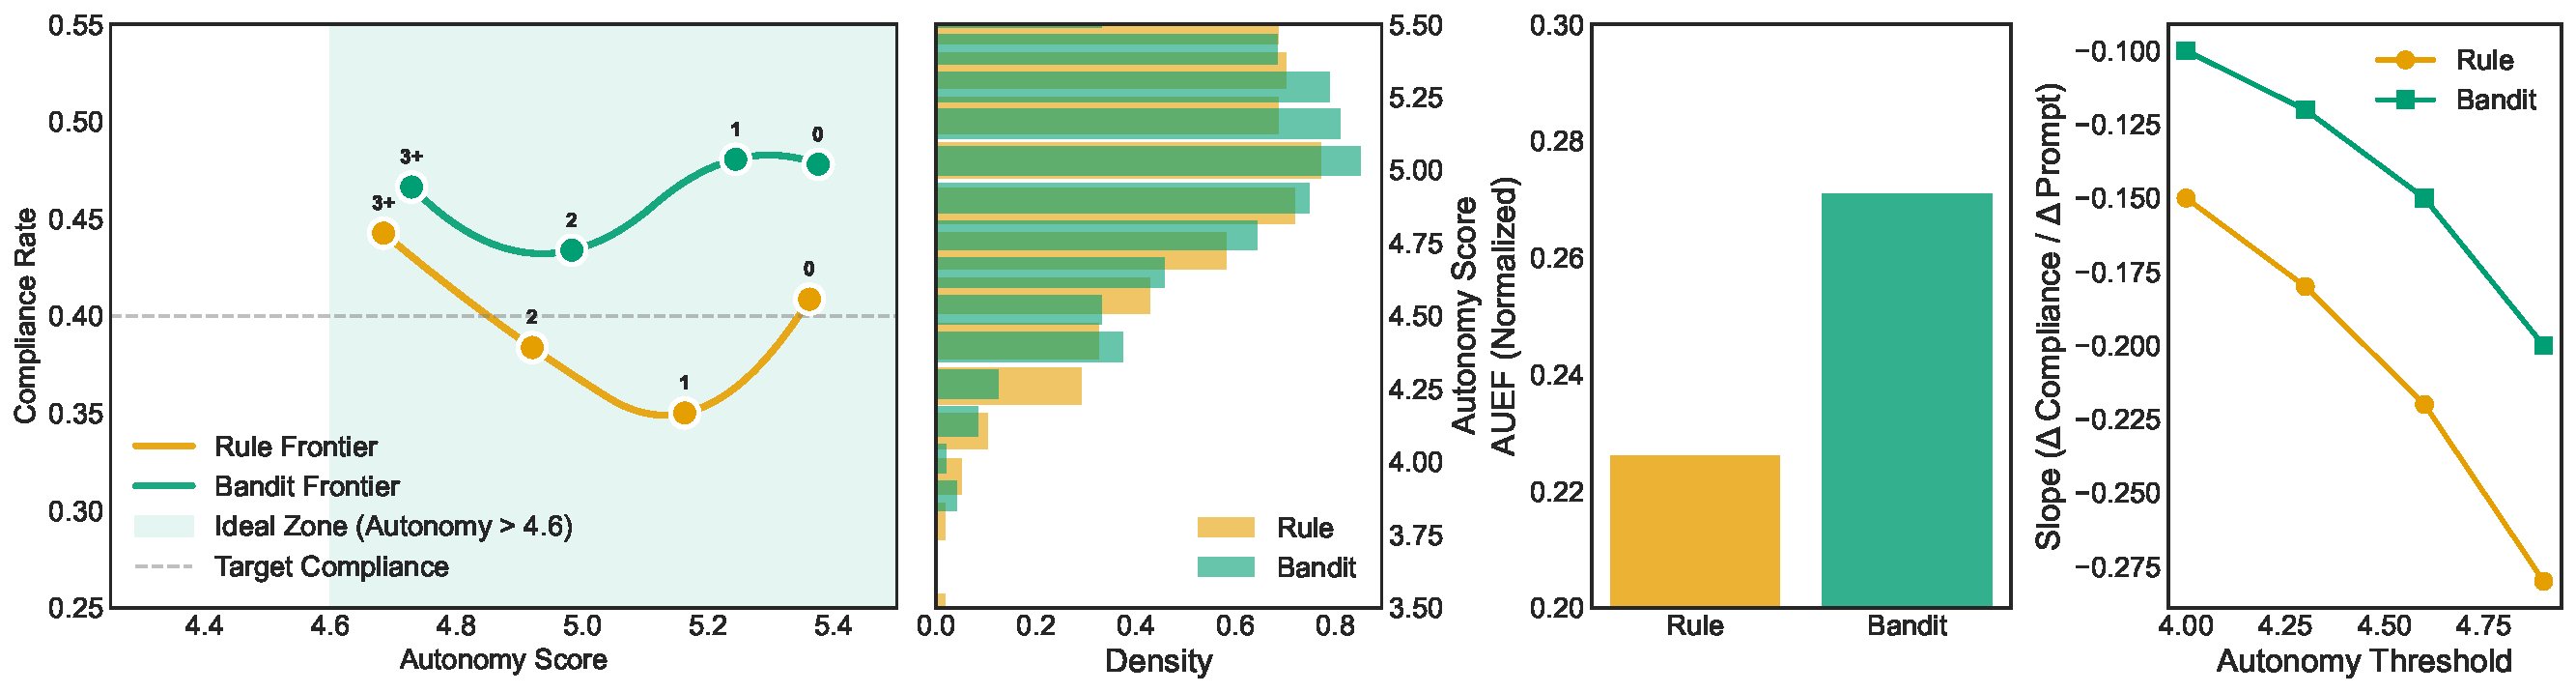
\includegraphics[width=0.7\linewidth, height=0.6\textheight, keepaspectratio]{assets/fig6_eef_enhanced.pdf}
\end{center}
\begin{columns}[T]
\begin{column}{0.56\textwidth}
\begin{keybox}[\faInfoCircle~~ What is the EEF?]
\scriptsize
The \textbf{Ethical--Efficacy Frontier} plots compliance (y-axis) against perceived autonomy (x-axis, 7-pt) across realized prompt intensities. By analogy to decision-curve analysis~[Vickers~2006], it visualizes the Pareto frontier of the autonomy--compliance trade-off.\\[3pt]
\textbf{Construction:} Bin participant-days by realized daily prompt intensity ($\{0,1,2,\ge3\}$), compute bin-wise means, fit LOESS (span=0.6) with isotonic monotonicity constraint. AUEF = normalized area under the frontier.
\end{keybox}
\end{column}
\begin{column}{0.42\textwidth}
\vspace{1pt}
\begin{findingbox}
\scriptsize
\textbf{AUEF:} Bandit \emphmark{0.271} vs Rule 0.226; diff +0.045 [0.018, 0.079], $p{=}.003$ (5{,}000 bootstrap reps)\\[3pt]
\textbf{At autonomy $\ge$4.6:} Streaming +6.1\,pp [1.6, 10.6]; Tabs +6.8\,pp [2.1, 11.5]\\[3pt]
\textbf{Endpoint autonomy (Week 2):} Bandit \emphmark{4.82} vs Rule 4.63; diff +0.19 [0.03, 0.35], $p{=}.021$\\[3pt]
\emphmark{Same compliance, more autonomy} --- the frontier shifts outward.
\end{findingbox}
\end{column}
\end{columns}
\end{frame}

% ============================================================

\begin{frame}{Persistence During Withdrawal --- RQ3}
\begin{columns}[T]
\begin{column}{0.6\textwidth}
\begin{center}
  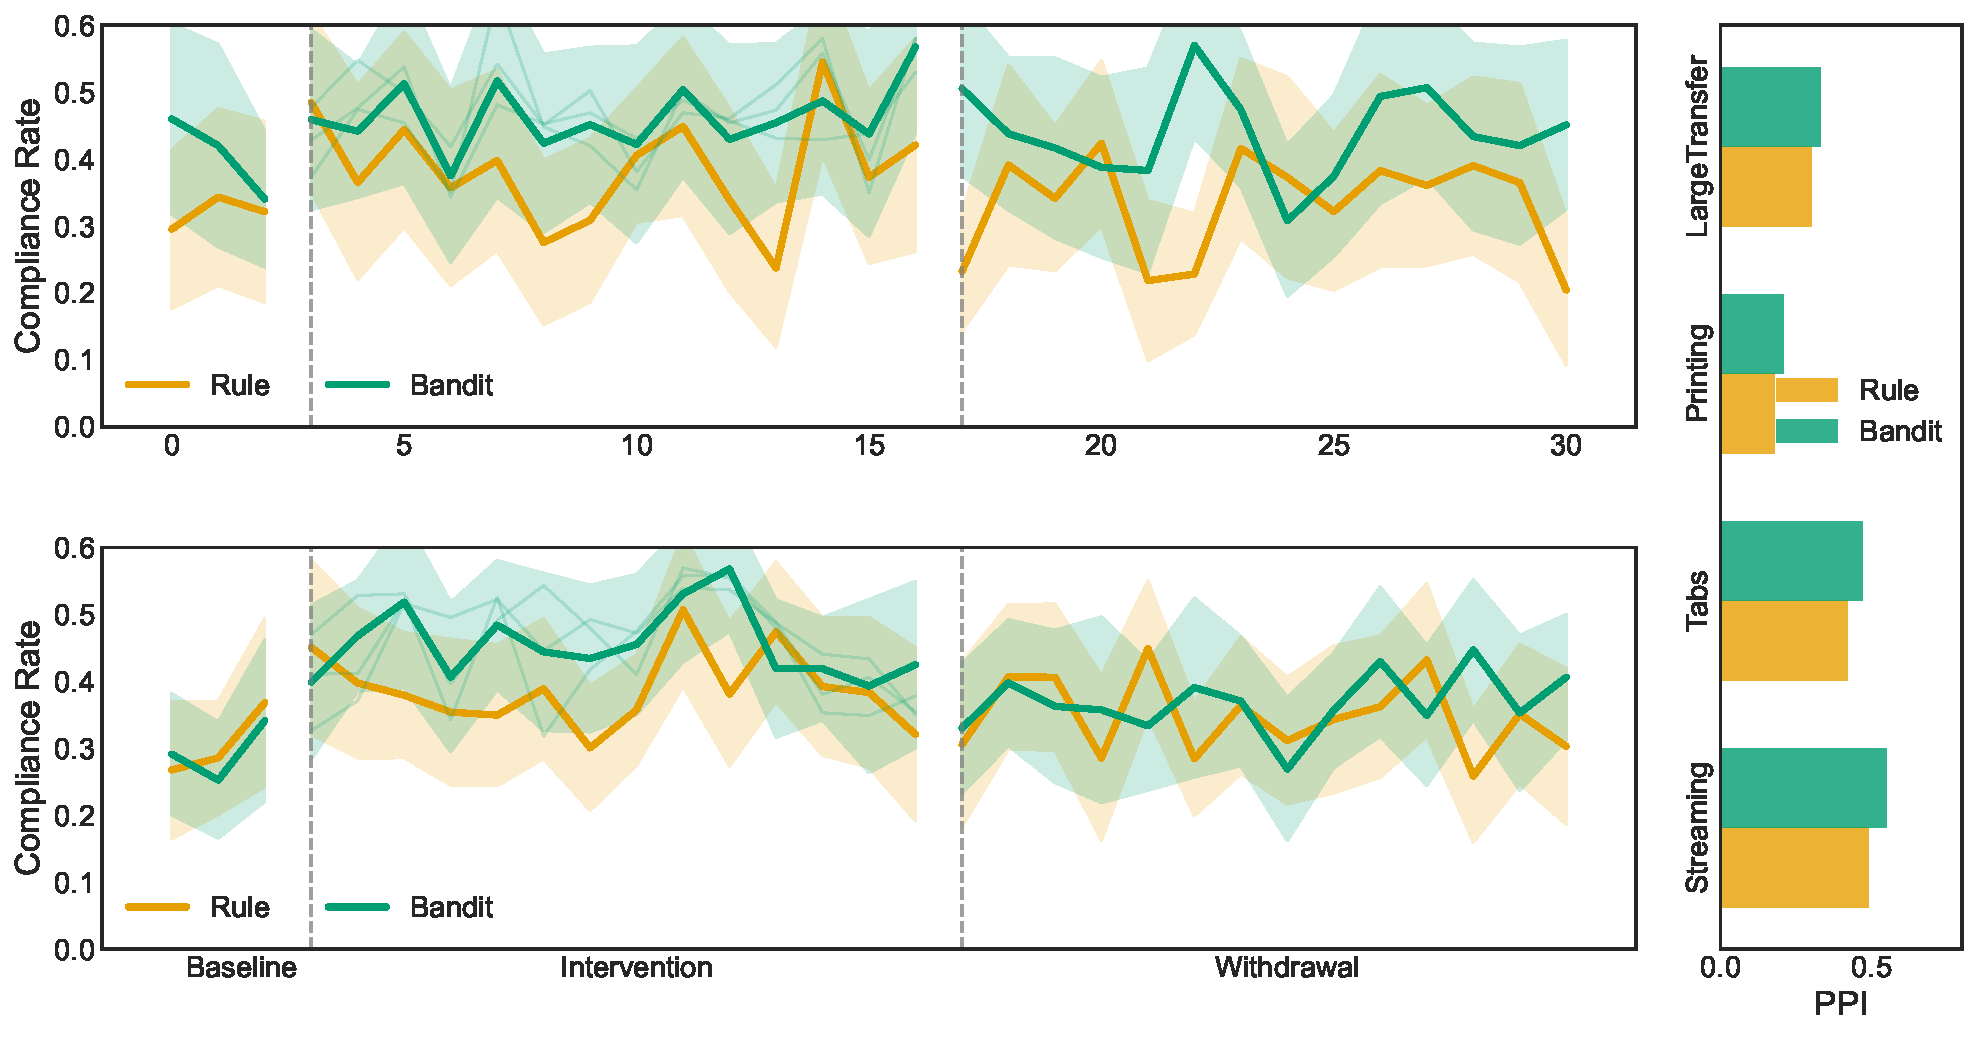
\includegraphics[width=\linewidth, height=0.76\textheight, keepaspectratio]{assets/fig7_aba_withdrawal_enhanced.pdf}
\end{center}
\begin{findingbox}
\scriptsize
\textbf{Week-5 Follow-up (micro-task probe):}\\
Streaming: Bandit +4.2\,pp [0.5, 7.9], $p{=}.028$\\
Tabs: Bandit +4.6\,pp [0.9, 8.3], $p{=}.015$\\[3pt]
\emphmark{Caveat:} Follow-up used scripted probes; estimates are an upper bound on retention. PPI is descriptive --- \textbf{not evidence of habit formation}. Longer deployments needed.
\end{findingbox}
\end{column}
\begin{column}{0.42\textwidth}
\vspace{1pt}
\begin{keybox}[\faClock~~ ABA(W) Withdrawal Results]
\scriptsize
\textbf{Partial Persistence Indices (PPI):}\\
(ratio of Withdrawal effect to Week-2 effect)

\vspace{3pt}
\renewcommand{\arraystretch}{1.1}
\begin{tabular}{@{}lcc@{}}
\toprule
\textbf{Behavior} & \textbf{PPI (mean)} & \textbf{Bandit $\Delta$} \\
\midrule
Streaming & 0.55 & +0.06--0.09 \\
Tabs      & 0.47 & +0.06--0.09 \\
Printing  & 0.21 & -- \\
Lg.\ Transfer & 0.33 & -- \\
\bottomrule
\end{tabular}

\vspace{3pt}
\scriptsize
Bandit consistently higher by 0.06--0.09 absolute across behaviors. High-frequency behaviors (streaming, tabs) show strongest partial persistence.
\end{keybox}
\end{column}
\end{columns}
\end{frame}

% ============================================================

\begin{frame}{Energy ROI --- RQ4}
\begin{columns}[T]
\begin{column}{0.50\textwidth}
\begin{keybox}[\faBolt~~ Energy Coefficients (literature-calibrated)]
\tiny
\renewcommand{\arraystretch}{1.15}
\begin{tabular}{@{}lll@{}}
\toprule
\textbf{Behavior} & \textbf{$\kappa_b$} & \textbf{Sensitivity} \\
\midrule
Streaming (HD$\to$SD) & 0.45 Wh/min & [0.25, 0.70] \\
Tabs (concurrency) & 0.20 Wh/tab$\cdot$hr & [0.10, 0.30] \\
Printing (skipped) & 30 Wh/print & [15, 60] \\
Lg.\ Transfer (GB) & 60 Wh/GB & [30, 100] \\
\bottomrule
\end{tabular}
\vspace{1pt}
$E_i^{\text{savings}} = \sum_b \Delta q_{i,b} \cdot \kappa_b$\\[2pt]
$\mathrm{ROI}_i = E_i^{\text{savings}} - E_i^{\text{overhead}}$
\end{keybox}
\vspace{3pt}
\begin{alertbox}[\faServer~~ On-Device vs Cloud Break-Even]
\tiny
$E_{\text{local}} \approx E_{\text{cpu}}^{\text{infer+update}} + E_{\text{idle}}$\\[2pt]
$E_{\text{cloud}} \approx E_{\text{device}}^{\text{rpc}} + E_{\text{net}} + E_{\text{server}}/N$\\[3pt]
Break-even at $\sim$5\,MB/day ($\sim$50\,kB per decision). For lightweight linear models with few prompts/day, on-device is \emphmark{no worse and often favorable}. Heavier models may flip the balance.
\end{alertbox}
\end{column}
\begin{column}{0.48\textwidth}
\begin{keybox}[\faCalculator~~ ROI Computation (Study 2, Bandit)]
\tiny
Using adjusted mean $\Delta$ from behavior-level outcomes:
\vspace{1pt}
\renewcommand{\arraystretch}{1.15}
\begin{tabular}{@{}lrl@{}}
\toprule
\textbf{Component} & \textbf{Value} & \\
\midrule
Streaming & $7.3 \times 0.45$ & = 3.29 Wh \\
Tabs & $0.5 \times 0.20 \times 8$h & = 0.80 Wh \\
Printing & $0.03 \times 30$ & = 0.90 Wh \\
Transfer & $0.05 \times 60$ & = 3.00 Wh \\
\midrule
\textbf{Gross savings} & & \textbf{7.99 Wh/day}\\
System overhead & & --0.30 Wh/day \\
\midrule
\textbf{Net ROI} & & \emphmark{$\sim$5.8 Wh/day} \\
\bottomrule
\end{tabular}

\vspace{1pt}
\textbf{Sensitivity:} [3.2, 9.1] Wh/day across coefficient ranges. Rule arm: $\sim$1.6 Wh/day lower.
\end{keybox}
\vspace{1pt}
\begin{findingbox}
\tiny
\textbf{Key finding:} Overhead $<$10\% of gross savings in all calibrations. Both arms net-positive. Bandit maintains positive margin across all sensitivity scenarios. \emphmark{Estimated net savings exceed system overhead by $\sim$19$\times$.}
\end{findingbox}
\end{column}
\end{columns}
\end{frame}

% ============================================================
%  SECTION 6: CONTRIBUTIONS
% ============================================================
{
\setbeamertemplate{footline}{}
\begin{frame}[plain,noframenumbering]
\begin{tikzpicture}[remember picture, overlay]
  \fill[chiTeal] (current page.north west) rectangle
    ([yshift=-3.5cm]current page.north east);
  \mosaicCorner{-6}{1.5}{1.5}
  \mosaicCorner{5.5}{1.0}{1.2}
  \node[anchor=west, text=white, font=\huge\bfseries]
    at ([xshift=16mm, yshift=-1.75cm]current page.north west) {6};
  \node[anchor=west, text=white, font=\Large]
    at ([xshift=28mm, yshift=-1.75cm]current page.north west)
    {Contributions \& Takeaway};
  \draw[chiAccent, line width=2pt]
    ([xshift=16mm, yshift=-2.8cm]current page.north west) --
    ([xshift=70mm, yshift=-2.8cm]current page.north west);
\end{tikzpicture}
\end{frame}
}

% ============================================================

\begin{frame}{Four Contributions}
\sideAccent
\vspace{4pt}
\begin{tikzpicture}[
  ctr/.style={rounded corners=4pt, text width=5.8cm, minimum height=2.6cm,
    align=left, font=\small, inner xsep=8pt, inner ysep=6pt, drop shadow}]
  \node[ctr, fill=chiTeal!8, draw=chiTeal!40] (c1) at (0,1.6) {
    \textcolor{chiTeal}{\faFlask~~\textbf{C1: Evaluation Rigor}}\\[3pt]
    {\scriptsize Parity-controlled, opportunity-denominator evaluation. Matched length/valence/budgets across arms; denominators include all detected opportunities regardless of delivery. Reduces content-length and selection-on-delivery confounds.}};
  \node[ctr, fill=chiAccent!6, draw=chiAccent!35] (c2) at (7,1.6) {
    \textcolor{chiAccent}{\faRobot~~\textbf{C2: On-Device Learning}}\\[3pt]
    {\scriptsize Privacy-preserving bandit with \textsc{DoNothing} as first-class action, user-governed quiet hours/budgets, and explicit in-situ feedback. Personalization without profiling: all features, models, and logs remain on device.}};
  \node[ctr, fill=chiGreen!6, draw=chiGreen!35] (c3) at (0,-1.6) {
    \textcolor{chiGreen!80!black}{\faBalanceScale~~\textbf{C3: New Lenses}}\\[3pt]
    {\scriptsize (i) Ethical--Efficacy Frontier (EEF): Pareto frontier relating compliance to autonomy (AUEF = 0.271 vs 0.226, $p{=}.003$). (ii) Energy ROI: net savings $\sim$5.8 Wh/day with sensitivity [3.2, 9.1]. On-device vs cloud break-even analysis.}};
  \node[ctr, fill=chiPurple!6, draw=chiPurple!30] (c4) at (7,-1.6) {
    \textcolor{chiPurple}{\faGlobe~~\textbf{C4: Field Evidence}}\\[3pt]
    {\scriptsize Two studies ($N{=}178$ + $N{=}54$) on tabs, streaming, large transfers, and printing. ABA(W) withdrawal data shows partial persistence (PPI 0.21--0.55). Week-5 follow-up retains Bandit advantage (+4.2--4.6\,pp).}};
\end{tikzpicture}
\end{frame}

% ============================================================

\begin{frame}{Five Design Principles (with Evidence)}
\sideAccent
\vspace{4pt}
\begin{tikzpicture}[
  dp/.style={rounded corners=3pt, text width=13cm, align=left, font=\small,
    inner xsep=8pt, inner ysep=5pt, drop shadow}]
  \node[dp, fill=chiTeal!7, draw=chiTeal!30] (d1) at (0,0) {
    \textcolor{chiTeal}{\faUserShield~~\textbf{1.\ Govern Intensity}} --- Quiet hours and prompt budgets as first-class constraints. {\scriptsize \textcolor{chiGray}{Evidence: autonomy slope $\hat{\eta}_1{=}{-}0.22$ pts/prompt ($p{<}.001$); cost accrues with \emph{intensity}, not tailoring ($p{=}.31$).}}};
  \node[dp, fill=chiAccent!5, draw=chiAccent!30, below=3pt of d1] (d2) {
    \textcolor{chiAccent}{\faEye~~\textbf{2.\ Make Targeting Legible}} --- ``Why this?'' explanations citing user goals and context. {\scriptsize \textcolor{chiGray}{Evidence: high-trust participants showed larger Bandit advantage (+8.7 vs +4.1\,pp at autonomy $\ge$4.6; interaction $p{=}.041$).}}};
  \node[dp, fill=chiGreen!5, draw=chiGreen!30, below=3pt of d2] (d3) {
    \textcolor{chiGreen!80!black}{\faLock~~\textbf{3.\ Minimize Data, Keep Local}} --- Personalization without profiling; all on-device. {\scriptsize \textcolor{chiGray}{No server profiles; ephemeral counters; overhead only 0.30 Wh/day ($<$10\% of gross savings).}}};
  \node[dp, fill=chiPurple!5, draw=chiPurple!25, below=3pt of d3] (d4) {
    \textcolor{chiPurple}{\faHandPaper~~\textbf{4.\ Learn Restraint}} --- \textsc{DoNothing} as first-class action. {\scriptsize \textcolor{chiGray}{DoNothing grew 38\%$\to$68\%; Wrong-time votes fell; temporal alignment improved (OR=0.86, $p{<}.05$).}}};
  \node[dp, fill=chiBlue!5, draw=chiBlue!25, below=3pt of d4] (d5) {
    \textcolor{chiBlue}{\faCalculator~~\textbf{5.\ Report Net Impact}} --- Energy ROI with assumptions and sensitivity bands. {\scriptsize \textcolor{chiGray}{Net ROI $\sim$5.8 Wh/day [3.2, 9.1]; overhead $<$10\% of savings; on-device favorable for lightweight models.}}};
\end{tikzpicture}
\end{frame}

% ============================================================

\begin{frame}{Limitations \& Threats to Validity}
\begin{columns}[T]
\begin{column}{0.48\textwidth}
\begin{alertbox}[\faExclamationTriangle~~ Study Design]
\scriptsize
\begin{itemize}\setlength\itemsep{3pt}
  \item \textbf{Short duration:} 2-week interventions with short pre-period. Supports within-participant adjustment but limits \emphmark{habit formation} claims. Withdrawal/follow-up probes are short-term only.
  \item \textbf{University-heavy sample:} recruited via university lists (43\%), community forums (17\%), online postings (40\%). Desktop/laptop Chromium users only --- may not generalize to mobile, IT-managed environments, or different cultural contexts.
  \item \textbf{Small Study 2 $N$:} $N{=}54$ is adequately powered ($\ge$80\% for 6--8\,pp differences) but limits subgroup analyses.
  \item \textbf{EEF is descriptive:} Realized intensity not randomized; co-varies with opportunity availability. Not causal.
\end{itemize}
\end{alertbox}
\end{column}
\begin{column}{0.50\textwidth}
\begin{alertbox}[\faExclamationTriangle~~ Measurement \& Energy]
\scriptsize
\begin{itemize}\setlength\itemsep{3pt}
  \item \textbf{Proxy-based energy estimates:} No direct device or network power metering. ROI uses literature-calibrated coefficients with sensitivity bands, not measured power.
  \item \textbf{Network electricity intensity:} Contested whether bit-proportional or capacity-dominated. We bracket both views with per-GB and capacity-bounded scenarios.
  \item \textbf{Print-to-PDF ambiguity:} Cannot disambiguate PDF exports from physical prints at browser level. May bias printing ROI component upward.
  \item \textbf{No rebound/spillover measurement:} Direct/indirect rebound and cross-domain spillovers remain out of scope. Longer deployments needed.
  \item \textbf{Architecture-dependent:} On-device favorable for lightweight models at low decision rates; heavier models may favor cloud.
\end{itemize}
\end{alertbox}
\end{column}
\end{columns}
\end{frame}

% ============================================================

\begin{frame}{Take-Home Message}
\begin{center}
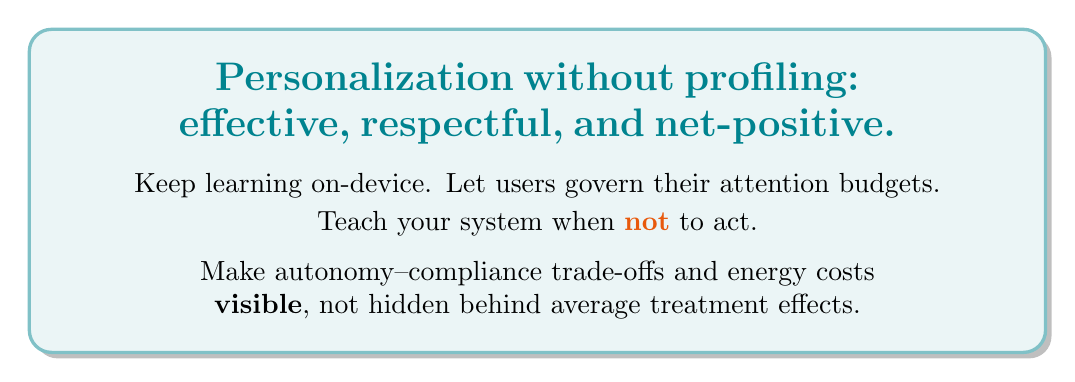
\begin{tikzpicture}
  \node[rounded corners=8pt, fill=chiTeal!8, draw=chiTeal!50, line width=1.2pt,
    inner xsep=20pt, inner ysep=12pt, text width=11.5cm, align=center,
    drop shadow] {
    {\Large\bfseries\textcolor{chiTeal}{Personalization without profiling:}}\\[3pt]
    {\Large\bfseries\textcolor{chiTeal}{effective, respectful, and net-positive.}}\\[8pt]
    {\normalsize
    Keep learning on-device. Let users govern their attention budgets.\\[2pt]
    Teach your system when \emphmark{not} to act.\\[6pt]
    Make autonomy--compliance trade-offs and energy costs\\
    \textbf{visible}, not hidden behind average treatment effects.}
  };
\end{tikzpicture}
\end{center}
\vspace{2pt}
\begin{columns}[T]
\begin{column}{0.48\textwidth}
\begin{findingbox}
\scriptsize
\textbf{Key numbers:}\\
Ctx--Gen: Streaming +8.0\,pp, Tabs +7.7\,pp (Study 1)\\
Bandit--Rule: Streaming +6.9\,pp, Tabs +7.2\,pp (Study 2)\\
AUEF: 0.271 vs 0.226 ($p{=}.003$); Net ROI $\sim$5.8 Wh/day
\end{findingbox}
\end{column}
\begin{column}{0.48\textwidth}
\begin{findingbox}
\scriptsize
\textbf{Resources:}\\
DOI: \texttt{10.1145/3772318.3791358}\\
Contact: Guangrui Fan --- fgr@tyust.edu.cn\\
$N{=}178$ (Study 1) + $N{=}54$ (Study 2)
\end{findingbox}
\end{column}
\end{columns}
\end{frame}

% ============================================================
%  THANK YOU
% ============================================================
{
\setbeamertemplate{footline}{}
\begin{frame}[plain,noframenumbering]
\begin{tikzpicture}[remember picture, overlay]
  \fill[chiDeep] (current page.north west) rectangle (current page.south east);
  \mosaicCorner{-6.5}{3.5}{2.0}
  \mosaicCorner{5.0}{3.0}{1.6}
  \mosaicCorner{-5.5}{-3.0}{1.4}
  \mosaicCorner{6.0}{-3.5}{1.8}
  \node[text=white, font=\Huge\bfseries] at ([yshift=12mm]current page.center)
    {Thank You!};
  \node[text=white!80, font=\large] at ([yshift=-2mm]current page.center)
    {Questions \& Discussion};
  \node[text=white!70, font=\small, text width=10cm, align=center]
    at ([yshift=-18mm]current page.center) {
    \faEnvelope~~fgr@tyust.edu.cn \qquad
    \faFile*~~DOI: 10.1145/3772318.3791358};
  \fill[white, opacity=0.92]
    ([yshift=0mm]current page.south west) rectangle
    ([yshift=16mm]current page.south east);
  \node[anchor=south west] at ([xshift=14mm, yshift=2mm]current page.south west)
    {
\includegraphics[height=1.1cm]{assets/tyust-logo.png}};
  \node[anchor=south] at ([xshift=-20mm, yshift=2.5mm]current page.south)
    {
\includegraphics[height=1.0cm]{assets/chi2026-logo.png}};
  \node[anchor=south] at ([xshift=20mm, yshift=2mm]current page.south)
    {
\includegraphics[height=1.0cm]{assets/acm-logo.png}};
  \node[anchor=south east] at ([xshift=-14mm, yshift=3mm]current page.south east)
    {
\includegraphics[height=0.9cm]{assets/sigchi-logo.png}};
\end{tikzpicture}
\end{frame}
}

\end{document}
